\chapter{TRIỂN KHAI HỆ THỐNG}

\section{Môi trường triển khai}

Hệ thống Chatbot được triển khai thực tế theo mô hình Client-Server nhằm đảm bảo sự phân tách rõ ràng giữa giao diện hiển thị và logic xử lý nghiệp vụ. Phía Client (Frontend) được xây dựng bằng thư viện ReactJS kết hợp với Tailwind CSS, mang lại giao diện người dùng hiện đại, tối giản và đáp ứng nhanh (responsive). Phía Server (Backend) sử dụng framework FastAPI của Python, cho phép xử lý các luồng dữ liệu bất đồng bộ (Asynchronous) hiệu quả, đặc biệt là khi phải thực hiện các tác vụ nặng như tạo Vector Embedding hay gọi API tới các mô hình ngôn ngữ. Toàn bộ dữ liệu Vector sinh ra từ tài liệu môn học được lưu trữ tập trung trên ChromaDB, đảm bảo tốc độ truy vấn tính bằng mili-giây. Lõi xử lý ngôn ngữ của hệ thống tận dụng sức mạnh của mô hình Gemini 2.5 Flash thông qua API, kết hợp chặt chẽ với cơ chế Retrieval-Augmented Generation (RAG) để đảm bảo câu trả lời luôn dựa trên tri thức nội bộ.

Về mặt tổ chức, mã nguồn được chia thành các module độc lập bao gồm: Giao diện người dùng (Frontend Sandbox), API xử lý nghiệp vụ (FastAPI Routers), Module RAG (xử lý Chunking \& Embedding), Vector Database (ChromaDB), Module Benchmark (chạy thử nghiệm tự động) và Dashboard thống kê (tổng hợp điểm số).

\section{Chức năng quản lý tài liệu}

Một trong những tiền đề quan trọng nhất của hệ thống RAG là việc xây dựng một kho tri thức phong phú và chất lượng. Chức năng quản lý tài liệu cho phép quản trị viên tải lên (Upload) các giáo trình, slide bài giảng định dạng PDF hoặc DOCX. 

\begin{figure}[H]
	\centering
	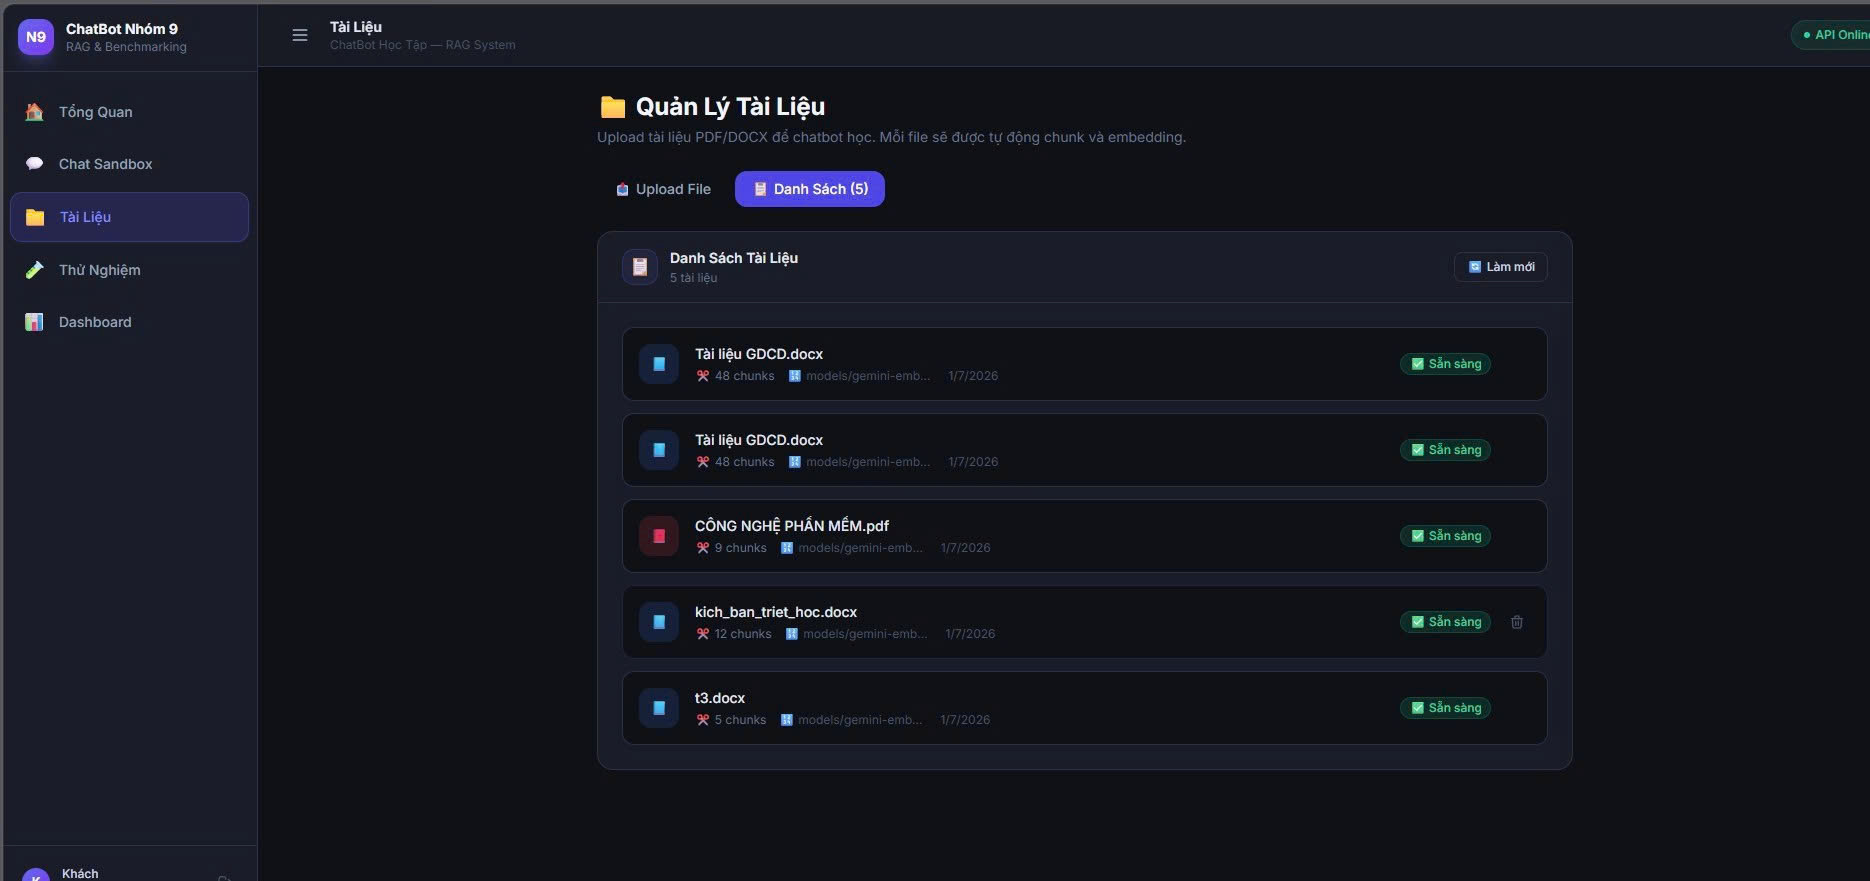
\includegraphics[width=\textwidth]{images/test_2}
	\caption{Chức năng quản lý tài liệu}
	\label{fig:document}
\end{figure}

Ngay khi tài liệu được tải lên hệ thống, Backend sẽ tự động kích hoạt một luồng xử lý văn bản (Ingestion Pipeline) phức tạp. Ban đầu, thư viện PyPDF hoặc pdfplumber sẽ quét qua toàn bộ tài liệu để trích xuất văn bản thô (raw text), loại bỏ các ký tự nhiễu và chuẩn hóa định dạng. Sau đó, văn bản thô này sẽ đi qua quá trình phân mảnh (Chunking). Hệ thống hỗ trợ nhiều chiến lược phân mảnh khác nhau (như Recursive Character Text Splitter) nhằm cắt tài liệu thành các khối (chunk) có độ dài tối ưu (thường từ 500 đến 1000 ký tự) mà vẫn giữ nguyên được ngữ cảnh của đoạn văn.

Tiếp theo, hệ thống sử dụng một mô hình Embedding (ví dụ: Google Gemini Embedding hoặc BAAI/bge-m3) để biến đổi các đoạn văn bản này thành các Vector đa chiều. Cuối cùng, các Vector này cùng với siêu dữ liệu (metadata như: tên file, số trang) được lưu trữ vào ChromaDB. Trạng thái của tài liệu sẽ được cập nhật thành "Sẵn sàng", lúc này người dùng có thể bắt đầu đặt câu hỏi liên quan đến nội dung tài liệu vừa tải lên.

\section{Chức năng Chat Sandbox}

Chat Sandbox là không gian làm việc chính của hệ thống, nơi sinh viên trực tiếp tương tác với AI thông qua việc đặt câu hỏi bằng ngôn ngữ tự nhiên. Giao diện này không chỉ đóng vai trò là một hộp thoại thông thường, mà còn là một môi trường thử nghiệm (Sandbox) cho phép người dùng tùy chỉnh các thông số kỹ thuật của RAG ngay trong thời gian thực.

\begin{figure}[H]
	\centering
	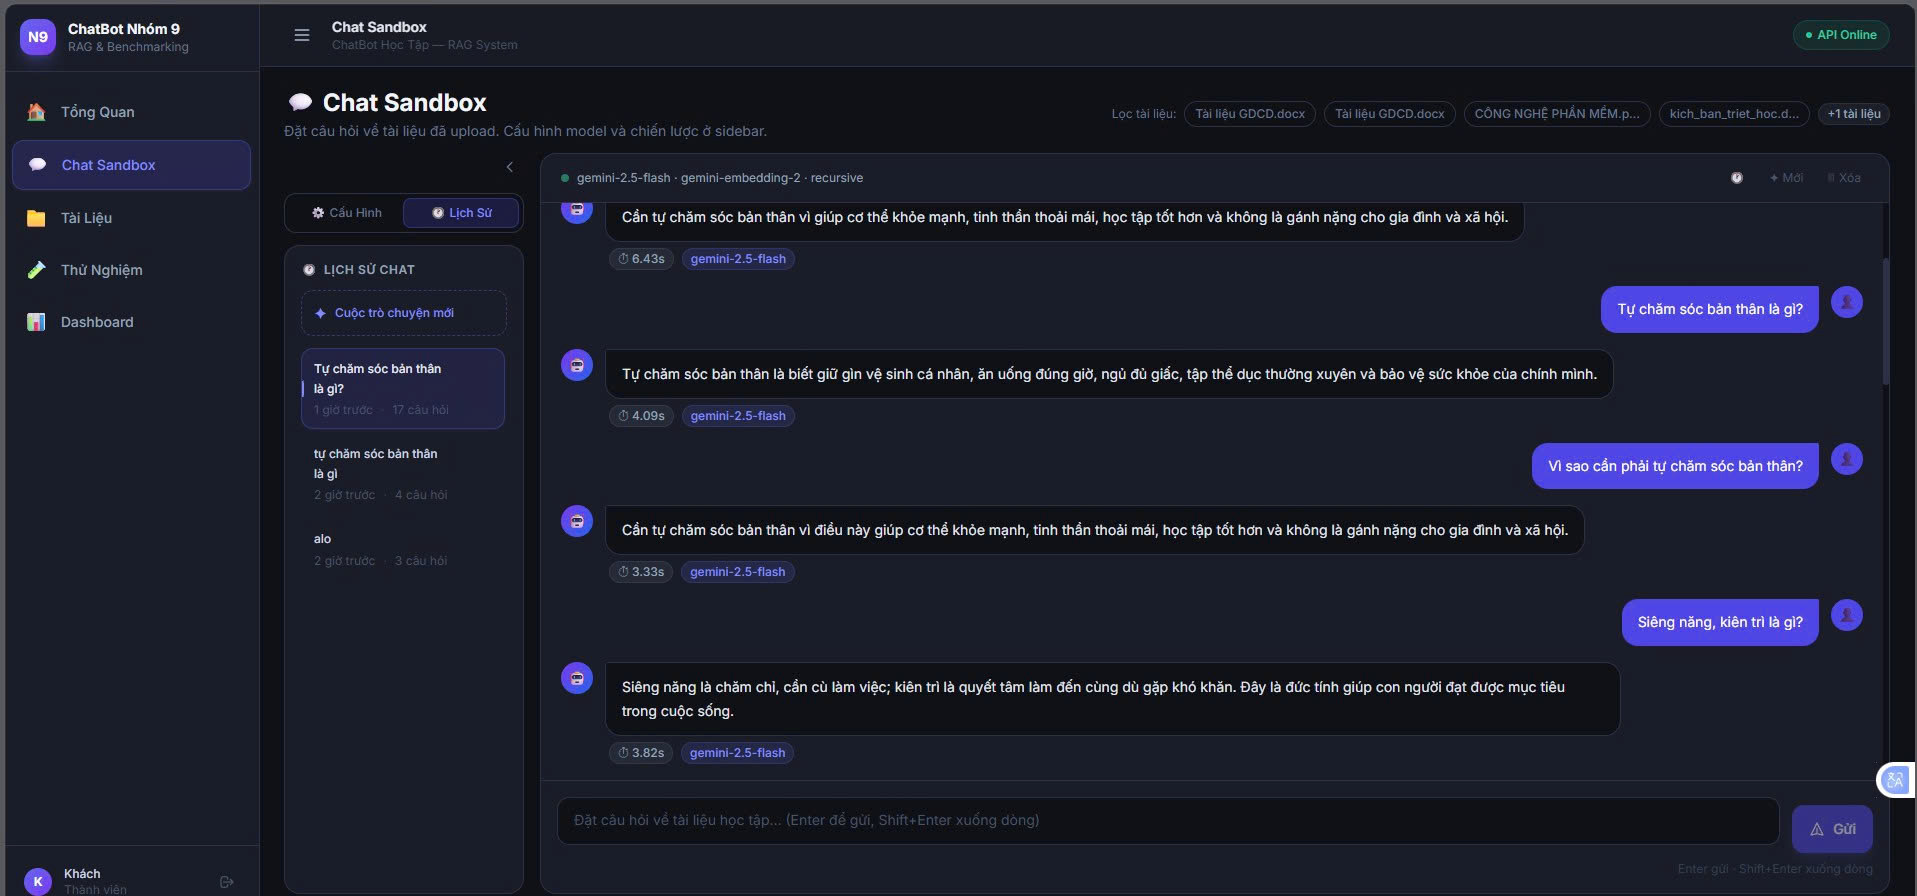
\includegraphics[width=\textwidth]{images/test_1}
	\caption{Giao diện Chat Sandbox}
	\label{fig:chat_sandbox}
\end{figure}

Giao diện hiển thị trực quan các thông số quan trọng như: mô hình AI đang được sử dụng (ví dụ: Gemini 2.5 Flash), thời gian trễ của API (Latency), cùng danh sách các tài liệu đang được chọn làm ngữ cảnh. Đặc biệt, người dùng có thể thiết lập hệ số Top-K (số lượng đoạn tài liệu liên quan tối đa được lấy ra từ database) hoặc thay đổi thuật toán Chunking ngay tại Sidebar. Chức năng lưu giữ ngữ cảnh hội thoại cũng được triển khai bằng cách truyền lại lịch sử tin nhắn trong các lần gọi API tiếp theo, giúp cuộc trò chuyện diễn ra tự nhiên và liền mạch mà không yêu cầu người dùng phải nhắc lại câu hỏi cũ.

\section{Luồng xử lý kỹ thuật của hệ thống RAG}

Để đảm bảo tốc độ và độ chính xác, luồng xử lý RAG từ lúc nhận câu hỏi đến khi trả về đáp án được thiết kế vô cùng chặt chẽ.

Đầu tiên, câu hỏi do sinh viên nhập vào sẽ được gửi qua REST API đến FastAPI. Tại đây, câu hỏi lập tức được đưa qua mô hình Embedding để sinh ra một Vector truy vấn (Query Vector). Vector này sau đó được chuyển cho ChromaDB để thực hiện thuật toán tìm kiếm khoảng cách tương đồng (như Cosine Similarity hoặc L2 Distance). ChromaDB sẽ duyệt qua không gian vector và trả về Top-K đoạn tài liệu (chunks) có ý nghĩa sát với câu hỏi nhất, bao gồm cả nội dung text và nguồn trích dẫn.

Ở bước tiếp theo, Backend tiến hành ghép nối (Augment) các đoạn tài liệu này vào một khuôn mẫu Prompt (Prompt Template) định sẵn. Mẫu Prompt này thường mang nội dung chỉ thị nghiêm ngặt, yêu cầu mô hình LLM (như Gemini) chỉ được phép sử dụng tri thức từ phần tài liệu đính kèm để trả lời, và nếu thông tin không có trong tài liệu, AI phải thông báo rõ ràng thay vì tự bịa đặt. Cuối cùng, Prompt hoàn chỉnh được gọi qua API tới LLM. LLM suy luận, tổng hợp thông tin, sinh ra câu trả lời và trả về giao diện Frontend, hoàn tất chu trình hỏi đáp một cách minh bạch và đáng tin cậy.

\section{Kết luận chương}

Chương này đã làm rõ quá trình triển khai hệ thống trong thực tế. Bằng việc phân tích sâu các luồng kỹ thuật từ quản lý tài liệu (Ingestion Pipeline) đến quá trình xử lý câu hỏi (Retrieval và Generation), có thể thấy hệ thống Chatbot được xây dựng không chỉ chú trọng về mặt giao diện mà còn tập trung giải quyết triệt để các bài toán tối ưu về tốc độ và tính toàn vẹn của dữ liệu trong mô hình RAG. Đây là cơ sở quan trọng để tiếp tục tiến hành các thử nghiệm Benchmark ở chương tiếp theo.